\documentclass[a4paper, 10pt]{article}

\usepackage{graphicx}
\usepackage{hyperref}

\hypersetup{
	colorlinks=true,
	linkcolor=blue,
	filecolor=magenta,
	urlcolor=cyan,
	citecolor=green,
}

%Replace title
\title{Stewart Platform Iteration 1 Standard Notes}
\date{\today}

\begin{document}
\maketitle

\pagebreak

\tableofcontents

\pagebreak


\section{Mechanical Design}
The goal being established is to the end of making the basic mechanical model of the Stewart platform. 

	\subsection{4/5/23}
		\subsubsection{Summary}
		Today was mostly research of the Stewart platform with some basic design. I found out that all Stewart platforms are termed rigid machines meaning their inverse kinematics solutions are significantly easier than forward. This means if we know the final position of the platform the math to determine angles of the actuators is easier than if we knew the angles of actuators and wanted the output. Study robotic kinematics further to understand these concepts. You may use either linear or rotary actuators, but the math will differ. The references and resources section contains some good examples and someone has done the math for control. Stewart platforms also use joint ends which are universal or spherical, this prevents the response and drive platforms from binding on each other and makes the math model simpler. 
		
		Some early design decisions that are more than obvious is the use of spherical joints, I believe I've found some cheap ones online. Further, a long horn on the driving servos will be chosen to maximize the travel of the driven platform; draw this out if you're confused: a platform where stub horns vs long horns are used. I'm also pretty confident I'll be using two triangular platforms which overlap like David's Star, with the driven triangle transitioning into a circular 'cage' housing for the LiDAR.
		
		\begin{figure} [h]
			\centering
			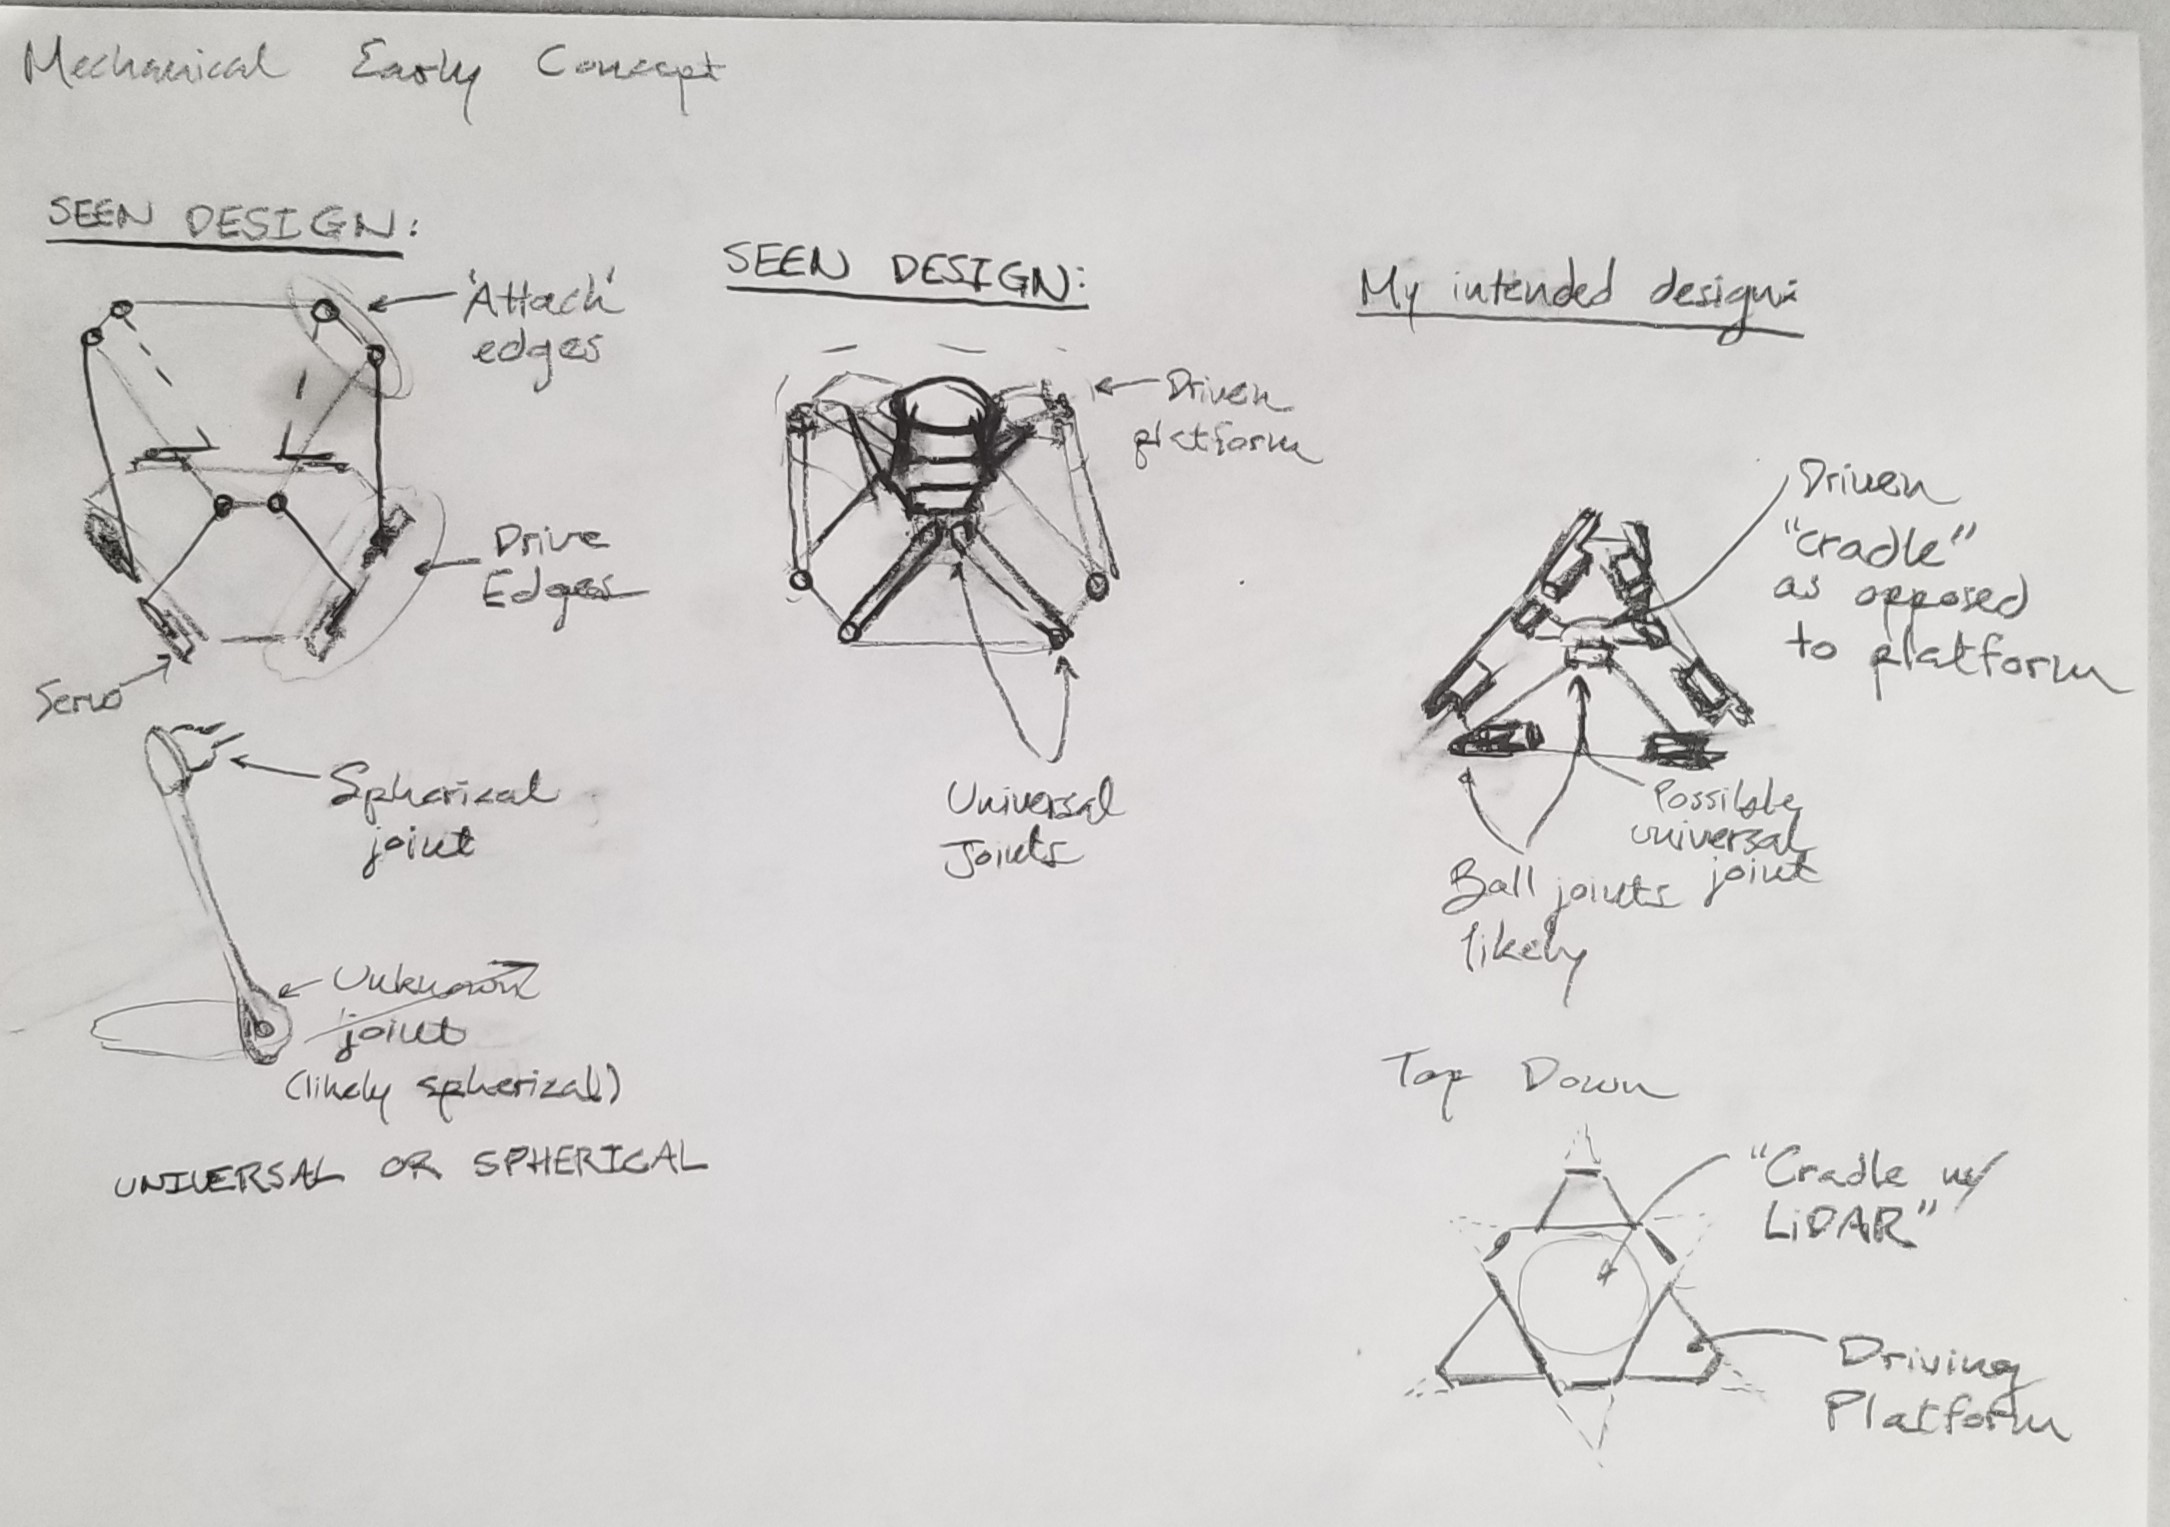
\includegraphics[scale=0.2]{early_mechanical}
			\caption{Mechanical sketches seen at the right}
			\label{fig_1}
		\end{figure}
	
		The first version of the eye will probably just be for practice controls and mechanical effectiveness. The first and final will share the same motors, joints, and most mounting; however, the final will include additional mounting for fixture to the rover, improved linkages, and additional components to make the whole assembly water/rubble resistant. 
		
	\subsection{4/6/23}
		\subsubsection{Summary}
		Continued research into the design of the Stewart platform. Notes on many of the design projects and research papers were completed in the 'Scratch Notes' document found in the drive. Perhaps in the future some notes summarizing the math and theory behind Stewart platforms can be written.
	
	\subsection{4/7/23}
		\subsubsection{Summary}
		Continued research, like yesterday.

	\subsection{References/Resources}
	\begin{itemize}
		\item A great example which includes a lot of mention of kinematics is seen \href{https://ntrs.nasa.gov/api/citations/19910007810/downloads/19910007810.pdf}{here}
		\item What might be called a treatise on Stewart platforms is found \href{https://www.ri.cmu.edu/pub_files/pub4/fong_terrence_w_1990_1/fong_terrence_w_1990_1.pdf}{here}
		\item An instructables on making a ghetto Stewart platform with Servos \href{https://www.instructables.com/Stewart-Platform/}{here}
		\item All robotic devices need kinematics models to work; \href{https://www.xarg.org/paper/inverse-kinematics-of-a-stewart-platform/}{this article} provides a kinematic model for Stewart platforms powered by rotary means (ie servo)
		\item Another good design example found \href{https://iopscience.iop.org/article/10.1088/1757-899X/563/5/052059/pdf}{here}
		\item Though it uses linear actuators, has some good examples of tests that might be performed on Stewart platforms \href{https://www.ncbi.nlm.nih.gov/pmc/articles/PMC6513003/}{here}
		\item Another good \href{https://core.ac.uk/download/pdf/322824733.pdf}{design example}
		\item A good \href{https://www.instructables.com/Six-Axis-Platform-Using-Linear-Actuators-Stewart-P/}{instructables}; however, this one uses linear actuators
		\item A good \href{https://www.ohio.edu/mechanical-faculty/williams/html/PDF/IndRob02.pdf}{design example} with potentially useful testing procedures
		\item A \href{https://www.mdpi.com/2218-6581/7/2/30}{lovely design} that looks nice and has a nice circular platform
		\item No tutorial, just great \href{https://www.youtube.com/watch?v=kscvCQTtVvw&t=0s}{inspiration}
		\item \textit{Parallel Robots} by J.P. Merlet
		\item \textit{Introduction to Robotics: Analysis, Control, Applications} by Saeed Niku
	\end{itemize}
	
	
\newpage	
	
\section{Electrical Design}
	\subsection{4/5/23}
		\subsubsection{Summary}
		Today some work was done in the way of planning the electrical; however, it relies all on existing knowledge of electronics. I may do more research in the future to ensure the the electrical is robust and end up changing the plans. Currently a solderable GikFun board will be used to provide all power and convey signal. Additionally, an Arduino Mega will be used for direct control of servos, but will recieve its instructions from the Nano. 
		
		Pins 2-7 on the Mega will convey logic through the GikFun board to the 6 movement servos, while pipns 10-11 will convey logic to the 'eyelids' of the protective housing. The GikFun will have a 5V barell jack that will recieve power from the PCB PDS of the rover. The Mega will recieve power from the GikFun, also a barell jack. The Mega will also be connected to the Nano via a standard USB printer cable. The Mega and Nano will communicate through ROS. An image below of the rough schematic can be seen.
		
		\begin{figure} [h]
			\centering
			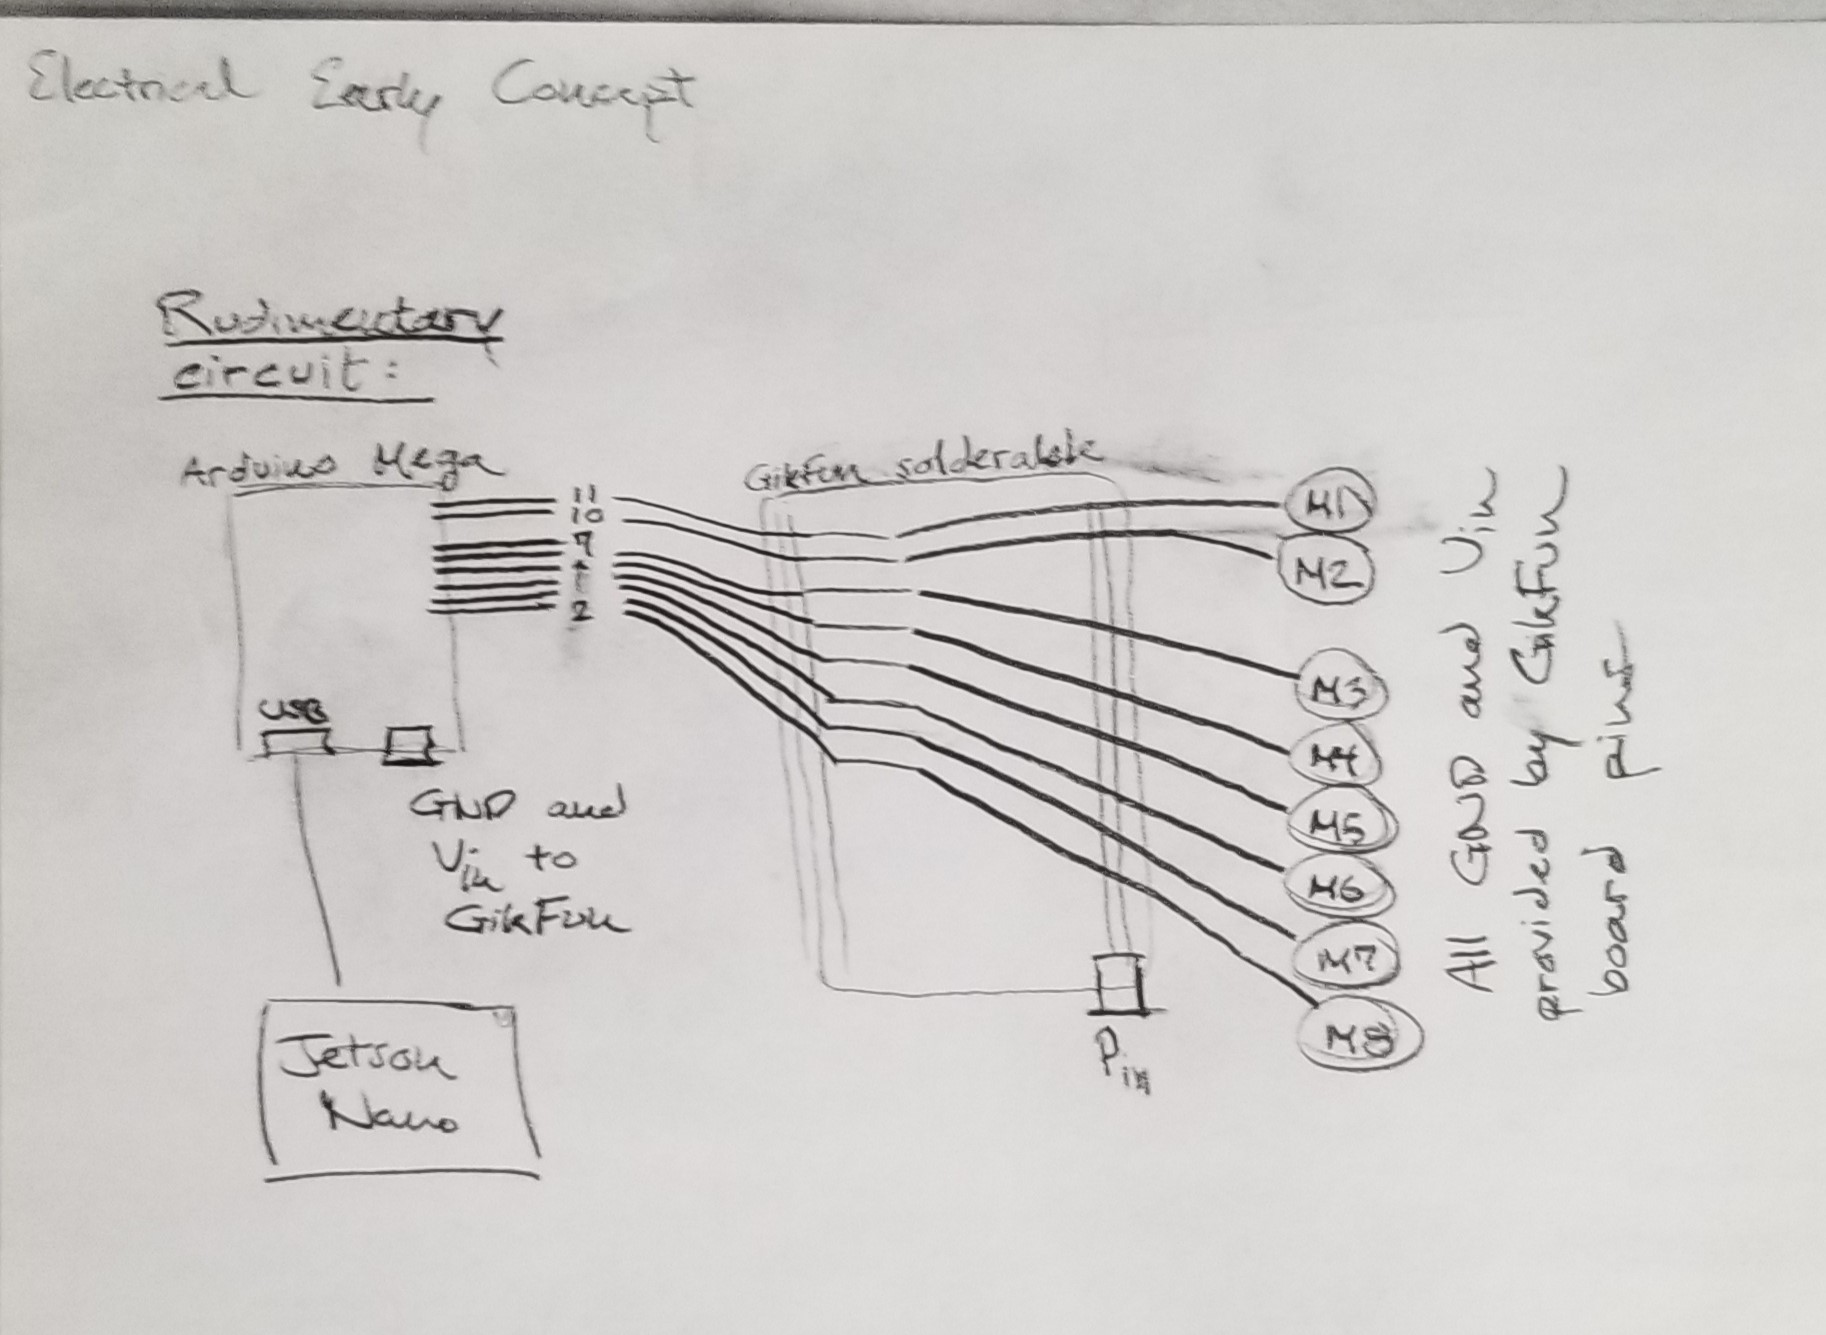
\includegraphics[scale=0.2]{early_electrical}
			\caption{Rudimentary electrical sketches}
			\label{fig_2}
		\end{figure}
		
	\subsection{References/Resources}

\end{document}